\documentclass[12pt,twoside]{article}
%%%%%%%%%%%%%%%%%%%%%%%%%%%%%%%%%%%%%%%%%%%%%%%%%%%%%%%%%%%%%
% Meta informations:
\newcommand{\trauthor}{Daniel Speck}
\newcommand{\trtype}{Seminar Paper} %{Seminararbeit} %{Proseminararbeit}
\newcommand{\trcourse}{Brain Modelling}
\newcommand{\trtitle}{Deep Learning: Neural Networks for Object Detection and Tracking Tasks}
\newcommand{\trmatrikelnummer}{632 13 17}
\newcommand{\tremail}{2speck@informatik.uni-hamburg.de}
\newcommand{\trarbeitsbereich}{Knowledge Technology, WTM}
\newcommand{\trdate}{29.05.2015}

%%%%%%%%%%%%%%%%%%%%%%%%%%%%%%%%%%%%%%%%%%%%%%%%%%%%%%%%%%%%%
% Languages:

% Falls die Ausarbeitung in Deutsch erfolgt:
% \usepackage[german]{babel}
% \usepackage[T1]{fontenc}
% \usepackage[latin1]{inputenc}
% \usepackage[latin9]{inputenc}	 				
% \selectlanguage{german}

% If the thesis is written in English:
\usepackage[english]{babel} 						
\selectlanguage{english}

%%%%%%%%%%%%%%%%%%%%%%%%%%%%%%%%%%%%%%%%%%%%%%%%%%%%%%%%%%%%%
% Bind packages:
\usepackage{acronym}                    % Acronyms
\usepackage{algorithmic}								% Algorithms and Pseudocode
\usepackage{algorithm}									% Algorithms and Pseudocode
\usepackage{amsfonts}                   % AMS Math Packet (Fonts)
\usepackage{amsmath}                    % AMS Math Packet
\usepackage{amssymb}                    % Additional mathematical symbols
\usepackage{amsthm}
\usepackage{commath}                    % Commath (e.g. \abs)
\usepackage{booktabs}                   % Nicer tables
%\usepackage[font=small,labelfont=bf]{caption} % Numbered captions for figures
\usepackage{color}                      % Enables defining of colors via \definecolor
\definecolor{uhhRed}{RGB}{254,0,0}		  % Official Uni Hamburg Red
\definecolor{uhhGrey}{RGB}{122,122,120} % Official Uni Hamburg Grey
\usepackage{fancybox}                   % Gleichungen einrahmen
\usepackage{fancyhdr}										% Packet for nicer headers
%\usepackage{fancyheadings}             % Nicer numbering of headlines

%\usepackage[outer=3.35cm]{geometry} 	  % Type area (size, margins...) !!!Release version
%\usepackage[outer=2.5cm]{geometry} 		% Type area (size, margins...) !!!Print version
%\usepackage{geometry} 									% Type area (size, margins...) !!!Proofread version
\usepackage[outer=3.15cm]{geometry} 	  % Type area (size, margins...) !!!Draft version
\geometry{a4paper,body={5.8in,9in}}

\usepackage{graphicx}                   % Inclusion of graphics
%\usepackage{latexsym}                  % Special symbols
\usepackage{longtable}									% Allow tables over several parges
\usepackage{listings}                   % Nicer source code listings
\usepackage{multicol}										% Content of a table over several columns
\usepackage{multirow}										% Content of a table over several rows
\usepackage{rotating}										% Alows to rotate text and objects
\usepackage[hang]{subfigure}            % Allows to use multiple (partial) figures in a fig
%\usepackage[font=footnotesize,labelfont=rm]{subfig}	% Pictures in a floating environment
\usepackage{tabularx}										% Tables with fixed width but variable rows
\usepackage{url,xspace,boxedminipage}   % Accurate display of URLs
\usepackage{wrapfig} % wrapped figures (with text floating around)
\usepackage{csquotes}
\input{insbox}

%%%%%%%%%%%%%%%%%%%%%%%%%%%%%%%%%%%%%%%%%%%%%%%%%%%%%%%%%%%%%
% Configurationen:

\hyphenation{whe-ther} 									% Manually use: "\-" in a word: Staats\-ver\-trag

%\lstloadlanguages{C}                   % Set the default language for listings
\DeclareGraphicsExtensions{.pdf,.svg,.jpg,.png,.eps} % first try pdf, then eps, png and jpg
\graphicspath{{./src/}} 								% Path to a folder where all pictures are located
\pagestyle{fancy} 											% Use nicer header and footer

% Redefine the environments for floating objects:
\setcounter{topnumber}{3}
\setcounter{bottomnumber}{2}
\setcounter{totalnumber}{4}
\renewcommand{\topfraction}{0.9} 			  %Standard: 0.7
\renewcommand{\bottomfraction}{0.5}		  %Standard: 0.3
\renewcommand{\textfraction}{0.1}		  	%Standard: 0.2
\renewcommand{\floatpagefraction}{0.8} 	%Standard: 0.5

% Tables with a nicer padding:
\renewcommand{\arraystretch}{1.2}

% Pagelength
\setlength{\textheight}{650pt}

%%%%%%%%%%%%%%%%%%%%%%%%%%%%
% Additional 'theorem' and 'definition' blocks:
\theoremstyle{plain}
\newtheorem{theorem}{Theorem}[section]
%\newtheorem{theorem}{Satz}[section]		% Wenn in Deutsch geschrieben wird.
\newtheorem{axiom}{Axiom}[section] 	
%\newtheorem{axiom}{Fakt}[chapter]			% Wenn in Deutsch geschrieben wird.
%Usage:%\begin{axiom}[optional description]%Main part%\end{fakt}

\theoremstyle{definition}
\newtheorem{definition}{Definition}[section]

%Additional types of axioms:
\newtheorem{lemma}[axiom]{Lemma}
\newtheorem{observation}[axiom]{Observation}

%Additional types of definitions:
\theoremstyle{remark}
%\newtheorem{remark}[definition]{Bemerkung} % Wenn in Deutsch geschrieben wird.
\newtheorem{remark}[definition]{Remark} 

%%%%%%%%%%%%%%%%%%%%%%%%%%%%
% Provides TODOs within the margin:
\newcommand{\TODO}[1]{\marginpar{\emph{\small{{\bf TODO: } #1}}}}

%%%%%%%%%%%%%%%%%%%%%%%%%%%%
% Abbreviations and mathematical symbols
\newcommand{\modd}{\text{ mod }}
\newcommand{\RS}{\mathbb{R}}
\newcommand{\NS}{\mathbb{N}}
\newcommand{\ZS}{\mathbb{Z}}
\newcommand{\dnormal}{\mathit{N}}
\newcommand{\duniform}{\mathit{U}}

\newcommand{\erdos}{Erd\H{o}s}
\newcommand{\renyi}{-R\'{e}nyi}
%%%%%%%%%%%%%%%%%%%%%%%%%%%%%%%%%%%%%%%%%%%%%%%%%%%%%%%%%%%%%
% Document:
\begin{document}
\renewcommand{\headheight}{14.5pt}

\fancyhead{}
\fancyhead[LE]{ \slshape \trauthor}
\fancyhead[LO]{}
\fancyhead[RE]{}
\fancyhead[RO]{ \slshape \trtitle}

%%%%%%%%%%%%%%%%%%%%%%%%%%%%
% Cover Header:
\begin{titlepage}
	\begin{flushleft}
		Universit\"at Hamburg\\
		Department Informatik\\
		\trarbeitsbereich\\
	\end{flushleft}
	\vspace{3.5cm}
	\begin{center}
		\huge \trtitle\\
	\end{center}
	\vspace{3.5cm}
	\begin{center}
		\normalsize\trtype\\
		[0.2cm]
		\Large\trcourse\\
		[1.5cm]
		\Large \trauthor\\
		[0.2cm]
		\normalsize Matr.Nr. \trmatrikelnummer\\
		[0.2cm]
		\normalsize\tremail\\
		[1.5cm]
		\Large \trdate
	\end{center}
	\vfill
\end{titlepage}

	%backsite of cover sheet is empty!
\thispagestyle{empty}
\hspace{1cm}
\newpage

%%%%%%%%%%%%%%%%%%%%%%%%%%%%
% Abstract:

% Abstract gives a brief summary of the main points of a paper:
\section*{Abstract}
Deep learning and the interrelated deep neural networks are one of the most successful learning strategies at the moment as the computing power for creating such structures rose in the past years via GPU computing. Image and video classification, object detection and tracking tasks can be fulfilled with these architectures which perform far better than more classical ones. One focus will be convolutional neural networks and the latest research on (mostly supervised) deep learning architectures.
  

% Lists:
\setcounter{tocdepth}{2} 					% depth of the table of contents (for Seminars 2 is recommented)
\tableofcontents
\pagenumbering{arabic}
\clearpage






%%%%%%%%%%%%%%%%%%%%%%%%%%%%
% Content:

% the actual content, usually separated over a number of sections
% each section is assigned a label, in order to be able to put a
% crossreference to it





\section{Introduction}
\label{sec:introduction}

Big data is a popular keyword in the last couple of years. With more and more devices being able to capture high-resolution images and videos, the data and information available on the internet increases rapidly, rather exponentially, but all this data is useless if this flood of information can not be searched, categorized and made easily accessible for humans. As a consequence of this situation classic, mostly static algorithms are \enquote{out-of-date} and new, intelligent systems have to be developed. Biological entities are, up to now, by far better when it comes to recognize, classify, sort etc. images or videos compared to computers. This circumstance led to researching intelligent systems that are able to adapt to their input, search for patterns and recognize, track and classify them.
\\
Inspired by biological systems, deep learning and especially convolutional neural networks have become popular because their results in classification and tracking tasks are state-of-the-art. In this paper a basic information view about artificial neural networks will be given for understanding the underlying concepts which are important to solve complex problems with machine learning architectures. In addition to that a comprehension of deep neural networks and deep learning will be made to point out the abilities but also the limits of \enquote{classic} neural networks. Also some information about the role of GPU-computing in such disciplines will be provided. For solving complex problems in classification, recognition, tracking etc. domains, convolutional neural networks have shown good performance in combination with GPU-computing, so they will be focused on. Especially the latest research on these topics and fields of application will be viewed in detail. An important contest for classification tasks is measuring the performance of such architectures with the ImageNet LSVRC databases and for videos with the YouTube 1M database by Google. Both topics will be introduced. One interesting fact is that pre-trained networks on videos showing sports did better on non-sports related video categorization than \enquote{fresh} networks. This is indicating an abstract, deep correlation between different domains in recognition tasks.





\section{Background information: Artificial neural networks}
\label{sec:ann}


Artificial neural networks are intended to approximate certain functions for machine learning purposes. They are intended to model learning processes. Fix/static algorithms can be calculated fast by modern computers but fail most times at disciplines requiring \enquote{intelligent} behavior. A classic example is recognizing handwritten digits because the shape, color and contrast highly vary in dependence of the used pencil and, of course, of the writing style. As a result, classic, static algorithms would fail to identify those varying patterns and therefore fail to appropriately classify handwritten digits. Such tasks can be fulfilled by artificial neural networks. A common architecture is the multilayer-perceptron as shown in figure \ref{fig:mlp1}.
\begin{wrapfigure}{r}{0.5\textwidth}
	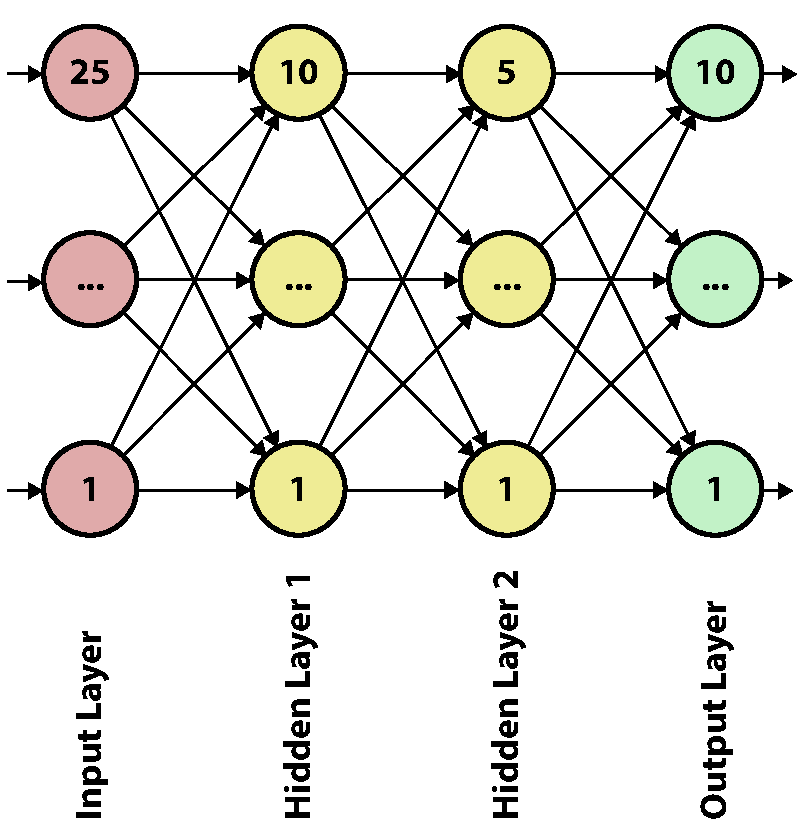
\includegraphics[width=0.5\textwidth]{neuralnet1.pdf}
	{\caption{An example of a classic, fully-connected multilayer-perceptron. The input layer holds 20 neurons, hidden layer 1 has 10 neurons, hidden layer 2 has 5 neurons and the output layer 2 neurons. All arrows but the short ones represent randomly initialized weights.}\label{fig:mlp1}}
\end{wrapfigure}
This artificial neural network, for example, could be used to classify handwritten digits. A database of hundreds of images would be needed for training the network accurately, using just a few training samples normally causes overfitting. The images information of input size 5x5, which results in 25 pixels, would be encoded by the 25 neurons in the input layer. The hidden layers would try to extract the features which are characteristic for each digit and the output layer with 10 neurons models the digits 0 to 9 for representing the calculated digit. Therefore each neuron of the output layer would give the probability for each digit (0-9) that it was this digit showing up in the input image. However, such architectures are insufficient for more complex tasks because they need a vast amount of resources, are not optimized and do not make use of any prior-knowledge of the problem. Non-deep structures where every layer is fully-connected turned out to be expensive in terms of computational resources and not optimal considering the results in disciplines of image and video classification, object recognition and tracking.






\section{Deep neural networks}
\label{sec:dnn}

Classic, small neural networks cannot succeed on complex tasks such as object detection in high-resolution, real world images. The variety of features, blurry backgrounds, one or several objects in an image and other factors render detection, tracking and classification tasks challenging. The ability to detect, track and distinguish real world objects demands complex structures with a much larger capability of solving complex problems. As computing power rises and GPU-computing became popular, neural networks are no longer limited to a few layers containing just some neurons. Modern solutions (in the year 2014) can carry tens of layers with thousands of neurons and millions of connections \cite{GoogleLargeScaleVideoClassification-Karpathy}. Complex structures like this enable computing complex problems which arise with tasks like image classification in real world images. To fulfill those assignments deep neural networks are used in combination with GPU-optimized code which is considerably faster than CPU-optimized code and hence allows larger, more accurate architectures \cite{MultiColumnDeepNeuralNetworksClassification-Ciresan}.





\section{Convolutional neural networks and image processing}
\label{sec:cnn}

For deep learning purposes (classic/fully-connected) multilayer perceptrons consume a sizable amount of resources for proper training when they are designed to solve complex tasks because the amount of neurons and especially weights increases rapidly with the network's size.
For example, a MLP like that showed in figure \ref{fig:mlp1} with four layers, an input layer with 25 neurons, two hidden layers with 10 and 5 neurons and an output layer with 10 neurons for classifying images with a size of 5x5 pixels into 10 different classes would have $25 * 10 + 10 * 5 + 5 * 10 = 350$ weights/connections. Training this net would already consume some time and space complexity. Compared to real world images such 5x5 images are tiny, even scaling this example up to images with a dimension of 50x50 is far less than real world images but would already result in an architecture like 2500 (input), 1000 (hidden), 500 (hidden), 10 (output) neurons\footnote{Assuming, for example, the task is classifying real hand-written digits}.
This architecture would have $2500 * 1000 + 1000 * 500 + 500 * 10 = 3,005,000$ weights/connections.
The human brain holds about 150 trillion ($1.5 * 10^{14}$) synapses \cite{AgingNeocortex-AmountOfSynapses}.
Moreover, as features in images capturing real world scenes are distributed in certain patterns (they cover spatially local correlation, such as shapes), there is no need to have every pixel's information being processed by one neuron. Actually in most cases results would be even better, if the pixel's information is pre-processed, for instance by edge detection filters. However a fully connected layer of neurons is not an optimal solution for this task.
\\
Convolutional neural networks (CNNs) are inspired by biology. Instead of connecting every pixels information directly with a neuron to process its information it filters the information in the first layers \cite{ImangeNetClassificationCNN-Krizhevsky}. This procedure is similar to the on processes happening when an biological eye receives stimuli.
The receptive field\footnote{\url{http://en.wikipedia.org/wiki/Receptive_field}} has a vast amount of photoreceptor cells\footnote{\url{http://en.wikipedia.org/wiki/Photoreceptor_cell}} gathering information and converging the received information on to distinctly fewer retinal ganglion cells\footnote{\url{http://en.wikipedia.org/wiki/Retinal_ganglion_cell}}. This process maps several features and reduces the input dimensionality as well as distinguishes the information to separate \enquote{channels} which are then transfered to the corresponding neurons to process features such as color, motion, shapes and so on separately \cite{DeepHierarchiesVisualCortex-kruger}.
\begin{figure}
	\centerline{
		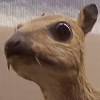
\includegraphics[width=0.3\textwidth]{animal-original.png}
		\qquad
		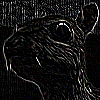
\includegraphics[width=0.3\textwidth]{animal-edge-detection.png}
	}
	{\caption{Left side: original image (greyscaled), right side: edge-detection kernel processed image. Original image by Michael Plotke, 28th of January, 2013. Open creative commons license.
			\protect\url{http://upload.wikimedia.org/wikipedia/commons/5/50/Vd-Orig.png} and \protect\url{http://upload.wikimedia.org/wikipedia/commons/6/6d/Vd-Edge3.png}}\label{fig:animal-edge-detection}}
\end{figure}
The idea of CNNs is based on this biological process: the information of an input image is convolved by several filters which try to extract interesting features in the first layer and in following layers this information is pooled and subsampled \cite{ImangeNetClassificationCNN-Krizhevsky}.
\\
Convolution itself is the repeated application of a function of the output of another function. In the context of CNNs it is applying different \enquote{filters} over an image to extract the already mentioned features. A convolution layer extracts the information of a pixel out of an image with kernels\footnote{\url{http://en.wikipedia.org/wiki/Kernel_(image_processing)}} \cite{ImangeNetClassificationCNN-Krizhevsky}.
\\
Example for one possible convolution layer: figure \ref{fig:animal-edge-detection} shows an image of an animal on the left side (original image, greyscaled) and a kernel-processed one on the right side. The used kernel matrix for filtering the left image is shown in equation (\ref{equation:kernal-matrix}).
\begin{wrapfigure}{r}{0.5\textwidth}
	\begin{equation}
		\label{equation:kernal-matrix}
		K_M =
		\begin{bmatrix}
		-1 & -1 & -1 \\
		-1 & 8 & -1 \\
		-1 & -1 & -1 \\
		\end{bmatrix}
	\end{equation}
\end{wrapfigure}
So basically each pixel's information in the right, processed image is the result of applying the kernel matrix $K_M$ (\ref{equation:kernal-matrix}) on the same pixel (and the neighboring pixels) in the left image. With a wide variety of different kernels several different features can be extracted from an image. Typical CNNs use tens to hundreds of different kernel filters gathering as many features from an image as possible. The resulting pixel processed by a kernel filter is calculated via the formula:
\begin{equation}
I_{out}(x,y) =
\abs{\sum_{a=1}^{3} \sum_{b=1}^{3} I_{in} (x+a-c_x, y+b-c_y) * K_M(a,b)}
\end{equation}

%\InsertBoxR{2}{
%	\parbox{0.5\textwidth}{
%		\small
%		\begin{gather}
%			\label{equation:example-kernel-processing}
%			\begin{split}
%				I_{in} =
%				\begin{bmatrix}
%				46 & 42 & 50 \\
%				44 & 65 & 56 \\
%				41 & 52 & 58 \\
%				\end{bmatrix}
%				\\
%				\\
%				I_{out}(2,2) = 131
%			\end{split}
%		\end{gather}
%		}}[3]
\begin{wrapfigure}[8]{R}{0.5\textwidth}
		\vspace{-20pt}
		\begin{gather}
		\label{equation:example-kernel-processing}
		\begin{split}
		I_{in} =
		\begin{bmatrix}
		46 & 42 & 50 \\
		44 & 65 & 56 \\
		41 & 52 & 58 \\
		\end{bmatrix}
		\\
		\\
		I_{out}(2,2) = 131
		\end{split}
		\end{gather}
\end{wrapfigure}
\noindent Where $c_x$ is the coordinate of the x-center and $c_y$ the coordinate of the y-center of the input image. After processing this filter to the whole image, edges would be highlighted and the rest becomes nearly black, like in figure \ref{fig:animal-edge-detection} (right side), so that shape features are extracted out of the original image.
Equation (\ref{equation:example-kernel-processing}) shows an example input and output of the image of figure \ref{fig:animal-edge-detection}. $I_{in}$ is the input with a dimension of 3x3 pixels extracted out of the original image. $I_{out}$ is the output for the center pixel ($x=2, y=2$) of the kernel-processed output image using the kernel filter $K_M$ of equation (\ref{equation:kernal-matrix}).
\\
Another idea of CNNs are subsampling layers, which follow convolutional layers. Subsampling reduces the overall amount of information and therefore not only saves resources for the later classification tasks but also strengthens the detected features in an image. Often max-pooling is used as a subsampling strategy in CNNs \cite{DeepNeuralNetworksObjectDetection-Szegedy, ImangeNetClassificationCNN-Krizhevsky} which determines the most distinctive pixel in a given area.
A max-pooling algorithm splits the input in grids and selects the maximum value out of each grid, thus non-maximal values are deleted so that only that information continues to exist which represents the current feature best \cite{GoogLeNet, ImangeNetClassificationCNN-Krizhevsky}.
Before applying max-pooling the input represents the presence of a feature in one or only some pixels. After this kind of dimensionality reduction the assertion is enlarged to a greater area, corresponding to several pixels of the original image. Szegedy et al. have made heavy use of this approach in \enquote{GoogLeNet} \cite{GoogLeNet}.
Additionally, this technique provides robustness to the position of a feature in an image, as the position becomes less important. Thereupon the extracted features are representing invariances, which are needed for classifying the collected information regardless of its position, rotation or scaling \cite{Invariances-Neural-Network-Khotanzad}.
The last layers of a CNN regularly consists of fully-connected layers. In comparison to feature extraction, strengthening and dimensionality reduction, those layers are supposed to take all gathered features/information and make predictions \cite{DeepNeuralNetworksObjectDetection-Szegedy, Multi-column-dnn-for-traffic-signs-ciresan, MultiColumnDeepNeuralNetworksClassification-Ciresan}. E.g. if the supplied input contains big shapes of ears, legs etc., filtered trunks, grey-ish color maps and so on, the fully-connected layers have to collect and mix all those gathered features/information and recognize it for finally classifying it as an image of elephants.



\section{Research and field of application}
\label{sec:research_and_application}


\subsection{Image classification}

For measuring the performance of a neural network top-1 and top-5 error rates have become popular \cite{ImangeNetClassificationCNN-Krizhevsky}. While letting a neural network classify some input test data the probabilities calculated by the network for each class are recorded. The error rates are arithmetic means of all test samples.
\begin{gather}
	\label{equation:top-1-error-rate}
	\text{top-1 error rate} =
	\frac{
		\displaystyle
		\sum_{S} x \;
		\begin{cases}
		1, & \text{if guessed class matches actual class of $S_i$} \\
		0, & \text{otherwise}
		\end{cases}}
		{|S|}
\end{gather}
\begin{gather}
	\label{equation:top-5-error-rate}
	\text{top-5 error rate} =
	\frac{
		\displaystyle
		\sum_{S} x \;
		\begin{cases}
		1, & \text{if the actual class of $S_i$ is one of the top 5} \\
		& \text{probabilities guessed by the neural network} \\
		0, & \text{otherwise}
		\end{cases}}
		{|S|}
\end{gather}
$S_i$ is the current test sample while S contains all test samples. If an architecture involves several independent CNNs, the predictions get averaged first and then follow the same procedure shown in equation (\ref{equation:top-1-error-rate}) and (\ref{equation:top-5-error-rate}).
Alex Krizhevsky et al. have shown in \enquote{ImageNet Classification with Deep Convolutional Neural Networks} \cite{ImangeNetClassificationCNN-Krizhevsky} the good performance of CNNs in image classification tasks. Their architecture achieved top-1 and top-5 error rates of 37.5\% and 17.0\% on the ImageNet LSVRC-2010 contest which was the best result in 2012.
The CNN consists of about $650,000$ neurons with $60$ million parameters and nine layers in total.
The only preprocessing made was resizing the images to a resolution of 256x256 because the images in ImageNet vary in resolution. Out of those images 224x224x3 dimensional patches are extracted. 224x224 in horizontal/vertical dimension and 3 different colors (RBG images). The first layer is a convolution layer which filters the input of 224x224x3 to a kernel map of 96 kernels with the size of 11x11x3 each. This slightly reduces the dimensionality of the input image and extracts 96 different features out of the input. Those features are anything that could be characteristic for the images.
The second layer is a max-pooling layer which filters the information via 256 5x5x48 kernels. Therefore the dimensionality is further reduced and already extracted features strengthened.
Afterwards convolutional and max-pooling layers follow the fifth layer until three fully-connected layers with 4096 neurons each try to collect and mix the information and then classify the images. The last layer has 1000 neurons representing the 1000 classes of ILSVRC, so a probability for each class is returned.
\\
One key problem with deep learning structures and especially CNNs is overfitting. Due to the size of those networks, a huge amount of training data is needed. An interesting method for reducing overfitting used by Krizhevsky et. al. is to design the first layer (224x224x3 for Krizhevsky's architecture) slightly smaller than the input data (256x256x3).
So instead of applying kernel filters on those input data (256x256x3) they first extract random 224x224x3 patches out of the original data.
This guarantees slightly different versions of each image when it is used for training the network and therefore extends the amount of training data.
Additionally they use horizontal reflections of those patches and altered the intensities of the RGB channels.
This technique can boost the number of available training data by a factor of hundreds or even thousands (depending on how many different color manipulated versions are used) \cite{ImangeNetClassificationCNN-Krizhevsky}.
\\
Another procedure to reduce overfitting and test errors is called \enquote{dropout} \cite{ImprovingNeuralNetworksDropout-Hinton-Krizhevsky}. The idea is to set the output of hidden neurons to zero with a certain probability, mostly $0.5$ \cite{ImangeNetClassificationCNN-Krizhevsky}. This prevents neurons of co-adapting to each other, which means that neurons can no longer distort their output, because they cannot \enquote{familiarize} anymore with some neurons of their parent layer and ignore others. With deactivating neurons randomly in each learning step the presence of another neuron is not guaranteed so neurons are more likely to learn and focus on robust features rather than on single attractive input neurons.
This has shown especially effective when applied in fully-connected layers \cite{ImangeNetClassificationCNN-Krizhevsky}.
\\
Normally the transfer function for a neuron's output is modeled as a hyperbolic tangent or sigmoid function, but those functions can increase the training time \cite{ImangeNetClassificationCNN-Krizhevsky}. Using Rectified Linear Units (ReLUs) \cite{RectifiedLinearUnits-Hinton} with a function like $f(x) = max(0, x)$ not only makes CNNs train a lot faster, but also slightly reduces the training error. Since low training error rates are reached faster (in less epochs) the whole network concentrates on robust features faster and this has an additional effect on convergence.
In Krizhevsky's architecture the 25\% error rate on the CIFAR-10 training dataset is reached six times faster with ReLUs than with classic hyperbolic tangent transfer functions \cite{ImangeNetClassificationCNN-Krizhevsky}.


\subsection{Video classification}

A more challenging and likewise interesting task is the classification of videos because instead of images where the input remains static the input of videos changes over time.
CNNs already showed state-of-the-art results in image recognition and classification tasks, so experiments with videos were just a matter of time. One problem was the changing of input over time in videos in combination with the long periods of training for CNNs. A solution figured out by a group of researchers of Stanford and Google was to improve the runtime performance. They split up the input data in two different streams, the \enquote{context stream} and the \enquote{fovea stream} to create a multiresolutional architecture \cite{GoogleLargeScaleVideoClassification-Karpathy}.
The original input dimension of this approach was 178x178. The fovea stream keeps track of the centered 89x89 pixels of a frame while the context stream analyzes the whole frame but downsampled to a size of 89x89 in total. Therefore the total input dimensionality is halved \cite{GoogleLargeScaleVideoClassification-Karpathy}. An illustration of this architecture is shown in figure \ref{fig:google-architecture-two-streams}.
\\
Four different solutions have been introduced by Karpathy et al. \cite{GoogleLargeScaleVideoClassification-Karpathy} to create CNNs capable of classifying videos properly: \enquote{Single Frame}, \enquote{Early Fusion}, \enquote{Late Fusion} and \enquote{Slow Fusion}.
\begin{itemize}
	\item Single Frame classification is an adoption already used for classifying images: only one image is being classified at a time.
	\item Early Fusion combines the pixel input information for a specific time window.
	\item Late Fusion calculates two different single frames which are combined at the last fully-connected layers.
	\item Slow Fusion is a mix of Early and Late Fusion: Several input images\footnote{The frames are consecutive in time.} pixel information  is combined and the streams are additionally combined every few layers. So it is achieved via extending the connectivity between the convolutional layers.
\end{itemize}
According to Karpathy et al. \cite{GoogleLargeScaleVideoClassification-Karpathy}, Slow Fusion had the best results with top-1 and top-5 error rates of 60.9\% and 80.2\%. This was reasonable, because the mix of single frame information with a variety of several input images over a specific time window in convolutional layers tries to extract features that are not only invariant for one frame, but robust over several frames and therefore stable over time.
Those features proved the best performance for videos. Besides the single frame performance showed surprisingly good results with 59.3\% for the top-1 error rate and 77.7\% for the top-5 error rate. This shows that motion cannot be a strong feature for video classification but rather a \enquote{supporting} feature for finetuning the error rates.

\begin{figure}
	\centerline{
		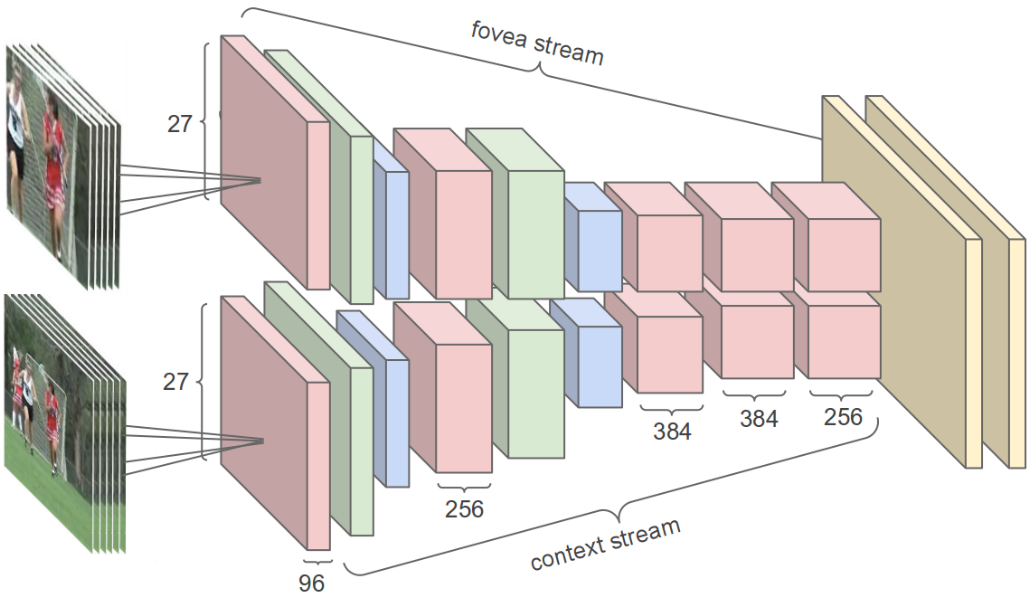
\includegraphics[width=0.95\textwidth]{google-architecture.png}
	}
	{\caption{CNN architecture by Karpathy et al. The input information is processed in parallel by the two streams. Graphics retrieved from \enquote{Large-scale Video Classification with Convolutional Neural Networks} by Andrej Karpathy et al. \cite{GoogleLargeScaleVideoClassification-Karpathy}}\label{fig:google-architecture-two-streams}}
\end{figure}

\begin{wrapfigure}{r}{0.5\textwidth}
	\vspace{-15pt}
	\centerline{
		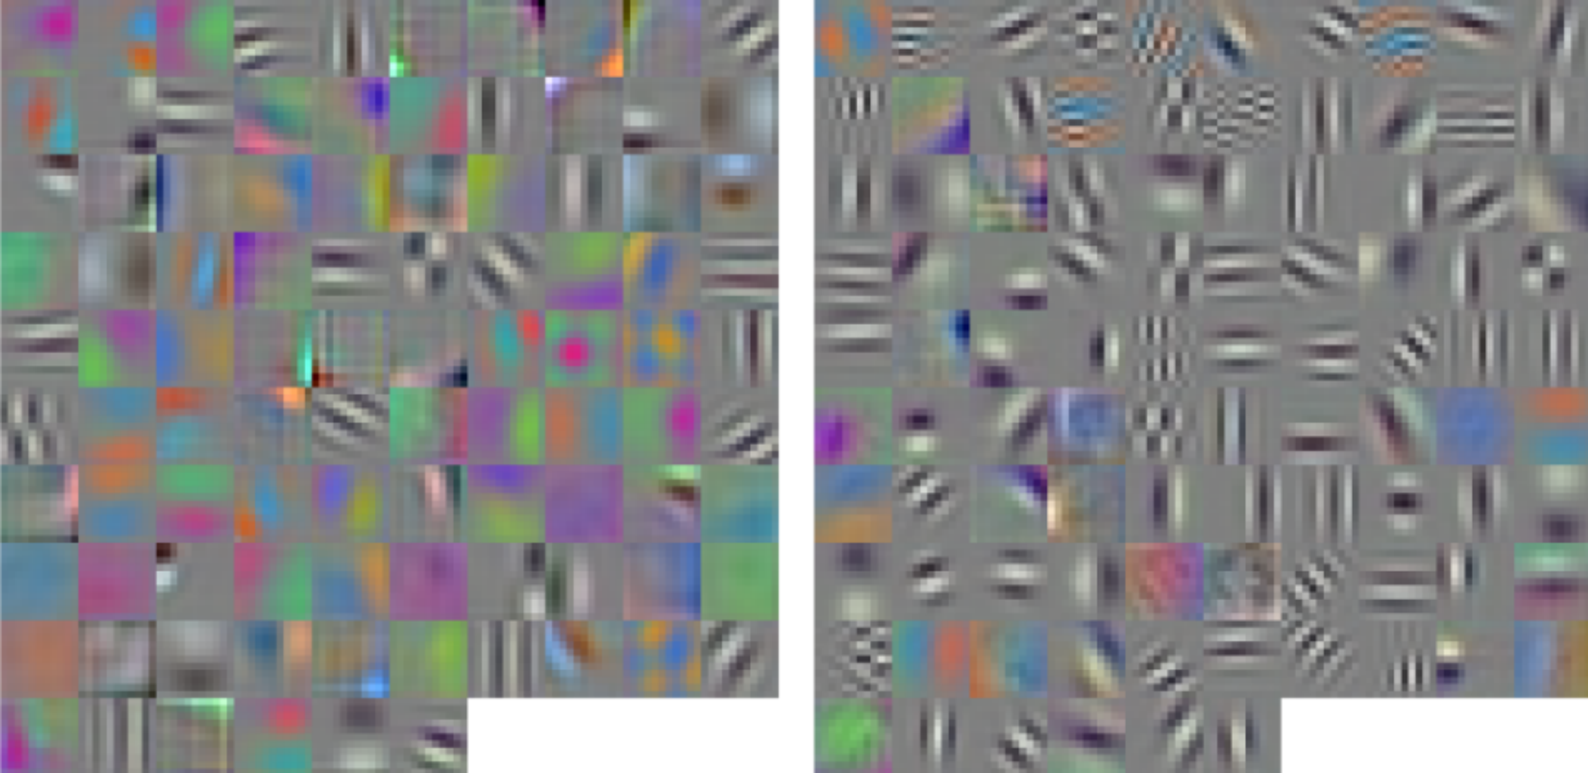
\includegraphics[width=0.5\textwidth]{GoogleVideoFilters.pdf}
	}
	{\caption{Filters of the first convolutional layer of the context stream (left) and fovea stream (right) after training. Graphics retrieved from \enquote{Large-scale Video Classification with Convolutional Neural Networks} by Andrej Karpathy et al. \cite{GoogleLargeScaleVideoClassification-Karpathy}}\label{fig:google-architecture-learned-filters}
		}
\end{wrapfigure}

\noindent The context stream and the fovea stream are focusing on different features. While the context stream is learning colors and overall low frequency features, which are more stable over time and do not alter heavily the fovea stream primarily focuses on greyscale and features with a high frequency \cite{GoogleLargeScaleVideoClassification-Karpathy}. This is shown in figure \ref{fig:google-architecture-learned-filters}.
The learned features show that mostly robust, general features remain after training the network. Interestingly this robustness is not only limited to the domain which the network was trained for. For example, one experiment of Karpathy et. al. was to retrain the top 3 layers of their network\footnote{Originally, the network of Karpathy et. al. was solely trained with videos showing sports} with non-sports videos and compare it to an untrained network with the same architecture, but which was exclusively trained with non-sports videos. The original network performed better in total and also showed up with lower error rates in less epochs \cite{GoogleLargeScaleVideoClassification-Karpathy}. Aforementioned outcomes are indicating a faster learning process as well as better results for pre-trained networks when retraining them for previously unfamiliar domains. This leads to the idea of specific domains becoming less important during a training process, especially in the back layers of an artificial neural network. Consequently the network tries to focus on generic features for recognizing objects rather than limiting on domain specific characteristics.






\subsection{Object tracking}

Object tracking in videos is an even more complex scenario because some object in a video has to be recognized and followed by its position over time. Varying background, changing in the lighting, unexpected motions etc. render this a challenging task.
Another complicating factor of tracking objects visually in terms of learning is the presence of only one training instance, especially when there is no prior knowledge to the object that should be tracked \cite{LearningDeepCompactImageTracking-Wang}. Obviously, when an architecture consists of a single, supervised network this fact would highly boost overfitting.
Generally existing tracking solutions use generative or discriminative approaches \cite{GenerativeDiscriminativeTrackerBook}. Generative trackers try to identify an object and collect robust features of it. After this process is finished a generative tracker extrapolates any possible object in a later scene and calculates the probability that for each object being the original object. So basically the intention is to find characteristic features and learn them for relocating it later on in another scene with a certain probability.
Contrary to this scenario discriminative trackers mainly focus on the differences between an object that should be tracked and the background, therefore they try to find features supporting to distinguish between the object and its background information \cite{GenerativeDiscriminativeTrackerBook}.
As a consequence discriminative trackers are more successful, when image distortion, changing backgrounds, rapidly changed lighting and other background and object effecting alterations appear whereas generative trackers perform better in consistent environments due to their highly adaption to object specific features in those scenes \cite{GenerativeDiscriminativePerformanceBenchmark}.
\\
Particle filters are a commonly used technique for both, preprocessing data or finetuning the filter itself for tracking purposes. A particle filter analyzes an object and creates state vectors to keep track of certain distributions of features over time. Hence, such a filter can model objects, e.g. with the distribution of colors, and keep track of them \cite{ParticleFilterObjectTracking}. 
One supposed solution for modern object tracking by Wang et. al. \cite{LearningDeepCompactImageTracking-Wang} is to combine preprocessing via particle filters with a mix of generative and discriminative trackers and neural networks. Before training or processing whole videos, they use 1 million randomly selected images out of a database of 80 million images to train a stacked denoising autoencoder. This procedure characterizes generic features of various domains, hence the problem of overfitting due to few training samples of one object that should be tracked is highly reduced. So the stacked denoising autoencoder learns common features of a large dataset. Subsequently the learned features can be extracted out of the encoding part of the stack denoising autoencoder and used for training the classification part of the neural network \cite{LearningDeepCompactImageTracking-Wang}. In addition to reduce overfitting it enables the neural network to differentiate between object features and background information, so this can be considered a learning alternative to classic discriminative trackers. If the scene changes significantly new features can be learned with the stacked denoising autoencoder readapting for the new scene. Once characteristic features are extracted, the neural network can be retrained with those features to ensure a better classification. For fulfilling this task the particle filter preprocesses each new frame and if the overall probability of formerly learned features comes below a certain, fixed threshold the scene is considered drastically changed and therefore the stacked denoising autoencoder and the neural network are retrained. Since the particle filter focuses on specific features of an object in the video this approach can be considered the generative tracker part.



\section{Conclusion}
\label{sec:concl}

The proposed approaches for object detection and tracking tasks demonstrate a large potential in the field of deep learning.
In the beginning of 2012 the best top-5 error rate on ImageNet was 16.4\% by \enquote{Team SuperVision} and in 2014 the best top-5 error rate was 6.67\% by \enquote{Team GoogLeNet} \cite{GoogLeNet}. This shows the rapid development of deep learning and CNNs but also that there is enough potential for even further improvement. At least for the next years the performance of humans in classifying images will be unmatched, which indicates that todays models have to be improved.
\\
In many papers \cite{GoogLeNet, DeepNeuralNetworksObjectDetection-Szegedy, ImangeNetClassificationCNN-Krizhevsky, LearningDeepCompactImageTracking-Wang, MultiColumnDeepNeuralNetworksClassification-Ciresan} researchers say improving the computational resources also improves machine learning architectures, because CNNs and other neural network architectures could deliver better results if they would be enlarged (which is not possible with current resources) but this would also require larger training data sets to prevent overfitting since overfitting increases when too complex architectures have too many parameters compared to the amount of available training data. Therefore new concepts, filters and architectures can improve machine learning and should be considered. One possible approach is combining several solutions like Wang et. al. did \cite{LearningDeepCompactImageTracking-Wang} with implementing a preprocessing step with a particle filter and combine different types of neural networks afterwards.
\\
On the one hand CNNs are one or maybe the most promising architecture at the moment \cite{GoogLeNet, ImangeNetClassificationCNN-Krizhevsky} with astounding results in classification tasks. Larger CNNs, more training data, enhanced precision and perhaps some architectural / mathematical improvements are likely to boost their performance even further.
On the other hand (although less resource demanding than fully-connected neural networks) their resource consumption is relatively high and as shown in \enquote{Deep Hierarchies In The Primate Visual Cortex} \cite{DeepHierarchiesVisualCortex-kruger} they are not equivalent nor equally effective as biological neural architectures. This displays that CNNs can only be a temporary model but not the ultimate solution and new architectures should be researched.
(CNNs vergrößern)
(biologische, visuelle Systeme haben weniger Layer)
(andere Architekturen?)




%%%%%%%%%%%%%%%%%%%%%%%%%%%%%%%%%%%%%%
% hier werden - zum Ende des Textes - die bibliographischen Referenzen
% eingebunden
%
% Insbesondere stehen die eigentlichen Informationen in der Datei
% ``bib.bib''
%
\newpage
\bibliographystyle{plain}
\addcontentsline{toc}{section}{Bibliography}% Add to the TOC
\bibliography{bib}


\end{document}


